
% Revisado por Juanan el día 12/03/2013

\srsfuncion{Consultar ficha empleado} \label{fun:consultarempleado}
	Esta función muestra la lista de empleados de la compañía, permitiendo buscar y filtrar resultados, así como información detallada de cada empleado en particular.
		
	\begin{enumerate}
		\item \textit{Prioridad}: alta.
		\item \textit{Entradas}
			\begin{enumerate}
				\item La lista de empleados se mostrará en orden alfabetico por apellidos por defecto, pero puede ordenarse según: nombre, NIF, fecha de nacimiento, tiempo trabajado en la empresa y departamento (Personal administrativo, Mecánico, Directivo, Personal de seguridad, Auxiliar de Vuelo y Piloto).							
			\end{enumerate}
		\item \textit{Flujo de operaciones}
			\begin{enumerate}
				\item Se muestra por pantalla una tabla con la lista de empleados ordenada por apellidos en orden alfabético. Se da la opción al usuario de ordenarla siguiendo los criterios mencionados anteriormente.
				\item Para cada empleado que seleccione el usuario se permite acceder a la información detallada de dicho empleado.
			\end{enumerate}
		\item \textit{Respuesta a situaciones no previstas}
			\begin{enumerate}
				\item Si no se puede acceder a la base de datos de empleados: se muestra por pantalla un mensaje de error indicando el error producido y se vuelve a la página principal del sistema.
				\item Si no se puede acceder a la información detallada del empleado: se muestra un mensaje por pantalla informando al usuario del error y vuelve a la pantalla anterior.
			\end{enumerate}
		\item \textit{Relación con otras funciones}\\
		La función está relacionada con \nameref{fun:editarempleado} y \nameref{fun:registrarempleado}.

	\end{enumerate}
	\begin{figure}[ht]\centering
	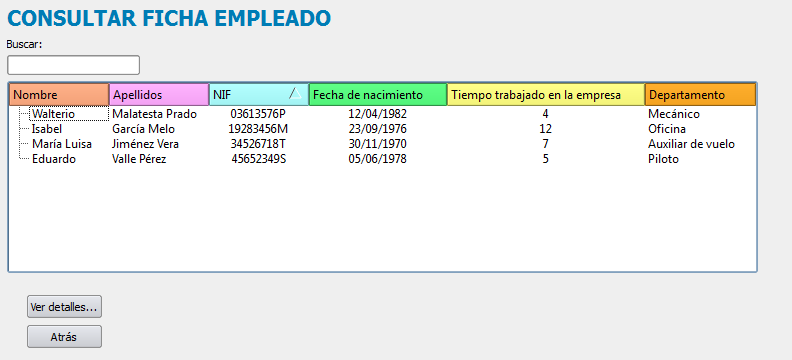
\includegraphics[scale=.6]{imagenes/consultarFichaEmpleadoImagen.png}
	\caption{Pantalla aproximada de la ficha de un empleado}
\end{figure}
								
